\classheader{2018-06-17}
\subsection*{Separable Equations}
\begin{definition-N}
Suppose for $y' = f(t, y)$ that $f(t,y) = g(t)h(y)$ for 2 functions $g(t)$, and $h(y)$. Then we say the ODE is \underline{separable}. (we can separate RHS into the product of 2 functions; one of $t$ alone and the other of $y$ alone).\\
\end{definition-N}
Then the ODE is $y' = g(t)h(y)$, and we can write...

\begin{equation*}
	\dfrac{1}{h(y)} \cdot \dfrac{dy}{dt} = g(t)\\
\end{equation*}
Since $y$ is a function of $t$, both sides are functions of $t$ and we can integrate \underline{wrt} $t$.
\begin{equation*}
	\underbrace{\int \bigg[\dfrac{1}{h(y)} \cdot \dfrac{dy}{dt}\bigg] dt}_{\text{the antiderivative of} \frac{1}{h(y)} \text{as a function of t}} = \underbrace{\int g(t) dt}_{\text{the antiderivative of }g(t)} \tag{$\star$}
\end{equation*}
The general solution to this kind of ODE is then found by integration alone.\\
\redhline\\
\begin{example-N}
	Find the general solution to $\dfrac{dy}{dx} = xy^2$. (Note: This ODE is separable, but \underline{NOT} linear!)\\
	\underline{Solution:} Separate the variables: $\dfrac{1}{y^2} \dfrac{dy}{dx} = x$. Then integrate both sides \underline{wrt} $x$:
	\begin{align*}
		\int \dfrac{1}{y^2} \dfrac{dy}{dx} = \int x dx\\
		-\frac{1}{y}  = \dfrac{x^2}{2} + c = \dfrac{x^2 + K}{2} \\
		\Rightarrow \boxed{y = \dfrac{-2}{x^2 + K}}
	\end{align*}
	\underline{Note:} While this is the general solution, particular solutions will require more than just a choice of $K$!\\
	This function works since for $y = \dfrac{-2}{x^2 + K}$\\
	\begin{equation*}
		y' = \dfrac{2}{(x^2 + K)^2}\cdot 2x = x\cdot (\dfrac{2}{x^2+K})^2 = x\cdot(\dfrac{-2}{x^2+K})^2 = xy^2
	\end{equation*}
\end{example-N}
\redhline
\subsubsection*{Notes}
\begin{enumerate}[label=\protect\circled{\arabic*}]
	\item The LHS of ($\star$) is interesting:\\\\
	$\int \bigg[\dfrac{1}{h(y)} \cdot \dfrac{dy}{dt}\bigg] dt$ is the antiderivative of $\dfrac{1}{h(y)}$ as a function of $t$; in the example,
	\begin{equation*}
		\int \bigg[\dfrac{1}{y^2} \cdot \dfrac{dy}{\bcancel{dx}}\bigg] \bcancel{dx} = \int \dfrac{1}{y^2} dy = \dfrac{-1}{y} + c
	\end{equation*}
	To see this, rewrite LHS ($\star$) using $u$ as the dependent variable:\\\\
	$\int\bigg[\dfrac{1}{h(u(x))} \cdot \dfrac{du}{dx}\bigg] dx$ looks just like the integrand one would find a substitution problem:\\
	Let $y=u(x), dy=u'(x)dx = \dfrac{du}{dx}dx$\\\\
	Then $\int\bigg[\dfrac{1}{h(u(x))} \cdot \dfrac{du}{dx}\bigg] dx = \int \dfrac{1}{h(y)} dy$ and we can integrate w.r.t. $y$ directly!\\
	Strictly speaking one \underline{does NOT} simply cross the dx's. But it does look that way.
	\item The book uses a slightly different formula:\\
	Any $y' = \dfrac{dy}{dx} = f(t,y)$ can be written as:
	\begin{equation*}
		M(x,y) + N(x,y)\dfrac{dy}{dx} = 0
	\end{equation*}
	(think $M = -f$ and $N = 1$, but this may sometimes not be the only way).\\
	Then if $M(x,y) = M(x)$ and $N(x,y) = N(y)$ we set\\
	\begin{equation*}
		M(x) + N(y)\dfrac{dy}{dx} = 0 \text{ or } N(y)\dfrac{dy}{dx} = M(x)
	\end{equation*}
	  and ODE is separable.
	 \item In differential form
	 \begin{equation*}
	 	M(x) + N(y)\dfrac{dy}{dx} = 0
	 \end{equation*}
	 may be presented as
	 \begin{equation*}
	 	M(x)dx + N(y)dy = 0 \text{ or } N(y)dy = -M(x)dx.
	 \end{equation*}
	 \begin{center}
	 Integrating the differentials yields.	
	 \end{center}
	 \begin{equation*}
	 	-\int M(x)dx = \int N(y)dy
	 \end{equation*}
	 \begin{example-N}
	 	We may sometimes see $y' = xy^2$ as $\dfrac{dy}{dx} = xy^2$ or $\dfrac{dy}{dx} - xy^2 = 0$, or $\dfrac{dy}{y^2} = xdx$\\
	 	The notation is different, but the ODE is the same.
	 \end{example-N}
	 \item Sometimes, a solution is known only implicitly:
	 \begin{center}
	 	\underline{Example in book:} \quad \quad $\mathlarger{\mathlarger{\dfrac{dy}{dx} = \frac{x^2}{1-y^2}}}$\\
	 	Solution is $\mathlarger{\mathlarger{\frac{-x^3}{3} + y -\frac{y^3}{3} = K}}$
	 \end{center}
	 
	\textbf{Question:} How does one use this information to find an explicit solution?\\
	\textbf{Question:} What is the domain of each solution?\\
	\textbf{Question:} How do we know which piece to pick?\\
	 \newline
	 For $y' = \frac{x^2}{1-y^2}$, $y(0) = 0$, the solution is $y(x)$ where $\dfrac{-x^3}{3} + y - \dfrac{y^3}{3} = 0$, but the function $y(x)$ is only defined up to the vertical tangent lines: These are where $y^2 = 1$ on $y = \pm 1$.\\
	 Here is where $\underline{y = 1}$, $\frac{-x^3}{3} + 1 -\frac{1}{3} \Rightarrow x = \sqrt[3]{2}$ and $\underline{y = -1} \Rightarrow x = -\sqrt[3]{2}$\\
	 \textbf{Caution:} A solution to an ODE is a function (even when defined implicitly) that \underline{includes its \textbf{domain!}}
	 \item Back to $y = xy^2$ with its general solution, $y(x) = \frac{-2}{x^2 + K}$. This is fine as a general solution.\\
	 But for an IVP, we will also need a domain for which the solution is continuous!
	 \begin{equation*}
	 	\textbf{IVP: } y' = xy^2, y(0) = 1
	 \end{equation*}
	 here the particular solution has $K$-value $K = -2$.\\
	 But $y(x) = \frac{-2}{x^2-2}$ does not solve $y' = xy^2, y(0) = 1$.\\
	 Only the \underline{continuous piece} that contains the initial value \underline{is} the solution.

	\begin{center}
	\begin{tikzpicture}
		\begin{axis}
		[xmin =-3, xmax = 3,
		ymin = -5, ymax = 5,
		axis lines = middle, samples=100]	
	
		\addplot[mark=none, draw=black, thin, domain=-1.40:1.40]{(-2)/(x^2 - 2)};
		\addplot[mark=none, draw=black, thin, domain=-4:-1.5]{(-2)/(x^2 - 2)};
		\addplot[mark=none, draw=black, thin, domain=1.5:4]{(-2)/(x^2 - 2)};
		\draw[dashed] ({axis cs:-1.41421356,0}|-{rel axis cs:0,0}) -- ({axis cs:-1.41421356,0}|-{rel axis cs:0,1});
		\draw[dashed] ({axis cs:1.41421356,0}|-{rel axis cs:0,0}) -- ({axis cs:1.41421356,0}|-{rel axis cs:0,1});

		\end{axis}
	\end{tikzpicture}
	\end{center}
	The solution to $y' = xy^2$, $y(0) = 1$ is $y(x) = \frac{-2}{x^2-2}$ on $(-\sqrt{2}, \sqrt{2})$ only.\\
	The solution to $y' = xy^2$, $y(2) = -1$ is $y(x) = \frac{-2}{x^2-2}$ on $(-\sqrt{2}, 0)$ only.\\\\
	The proper domain is absolutely necessary to specifying a solution.	 
\end{enumerate}
\begin{example-N}
	One last example:\\
	\begin{equation*}
		\text{Solve the IVP } ty' + 2y = 4t^2
	\end{equation*}
	\begin{center}
		for \circled{a} $y(-1) = 1$, \quad \circled{b} $y(-1) = 2$,\quad \circled{c} $y(0) = 0$,\quad \circled{d} $y(0) = 1$\quad 
	\end{center}
	\textbf{Solution: }Here method of integration factors gives us... $y(t)= t^2 + \frac{c}{t^2}$ as the general solution
	\begin{enumerate}[label=\protect\circled{\alph*}]
		\item $y(-1) = 1 = (-1)^2 + \frac{c}{(-1)^2} \Rightarrow c = 0$ \quad \quad $y(t) = t^2$ for $t \in (-\infty, \infty)$.
		\item $y(-1) = 2 = (-1)^2 + \frac{c}{(-1)^2} \Rightarrow c = 1$ \quad \quad $y(t) = t^2 + \frac{1}{t^2}$ for $t \in (-\infty, 0)$.
		\item Connect plus in 0. But the point $(0,0)$ is on an integral curve of IVP. It is on the curve $y = t^2$ on $(-\infty, \infty)$.
		\item The point $t = 0$, $y = 1$ is not on any integral curve. The IVP $ty' + 2y = 4t^2$, $y(0) = 1$ has \underline{no solution.} $\longrightarrow$ \underline{What gives??}\\
		\begin{center}
		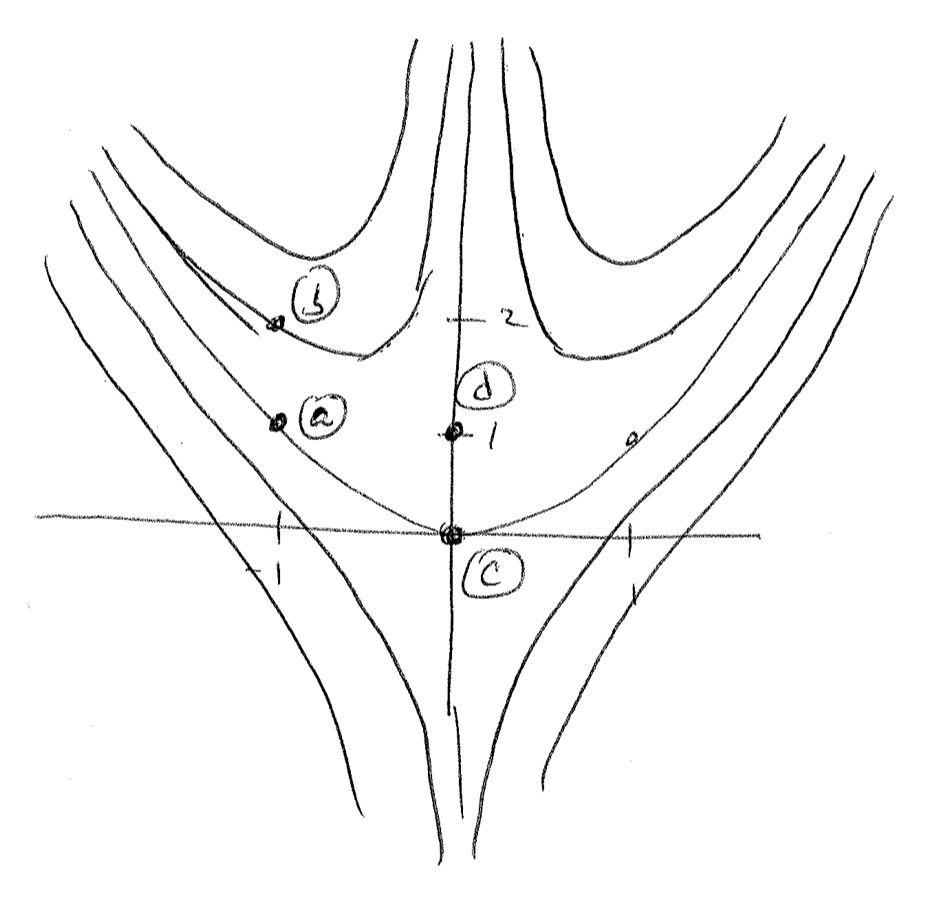
\includegraphics[width=10cm]{4-1}	
		\end{center}
		\begin{itemize}
			\item the domain of the IVP solution in \circled{a} is $(-\infty, \infty)$
			\item the domain of the IVP solution in \circled{b} is $(-\infty, 0)$
		\end{itemize}
		(This is only one piece of $ty(t) = t^2 + \frac{1}{t^2}$ the one that includes the point.)
		$\Rightarrow$ Solution to the IVP $ty' + 2y = 4t^2$, $y(0) = 1$ is
		\begin{equation*}
			\boxed{y(t) = t^2 + \frac{1}{t^2} \quad \text{ on } (-\infty, 0)}
		\end{equation*}
		\\
		\begin{center}
			\huge \underline{Careful here.}
		\end{center}
	\end{enumerate}
	
	 
\end{example-N}